\documentclass[letterpaper,12pt,fleqn]{article}
\usepackage{matharticle}
\usepackage{graphicx}
\pagestyle{plain}
\begin{document}

\begin{center}
\Large Math-08 Homework \#12 Solutions
\end{center}

\vspace{0.5in}

\underline{Reading}

\begin{itemize}
\item Text book section 3.1, 3.2
\end{itemize}

\underline{Problems}

Note that all sketches of graphs must have all found intercepts and
discontinuities labeled. All domains and ranges must be expressed in
interval notation. Remember, sketches do not have to be to scale!

\begin{enumerate}
\item Some kids are playing with a toy that launches balls straight up into
  the air. The balls leaving the launcher with a velocity of 96 ft/s. How high
  do the balls go?

  We start with the motion under gravity formula:
  \[h(t)=h_0+v_0t-16t^2\]
  This time, $h_0=0$ feet (on the ground) and $v_0=96$ ft/s:
  \[h(t)=96t-16t^2\]
  
  \begin{enumerate}
  \item Find the answer by completing the square.

    \begin{eqnarray*}
      h(t) &=& -16(t^2-6t) \\
      &=& -16(t^2-6t+9)+16(9) \\
      &=& -16(t-3)^2+144 \\
    \end{eqnarray*}

    This is an inverted parabola with vertex at $(3,144)$. Thus, the ball
    reaches its maximum height of 144 feet after 3 seconds.
    
  \item Find the answer using the $-\frac{b}{2a}$ shortcut.

    $x=-\frac{96}{2(-16)}=\frac{96}{32}=3$ \\
    $y=96(3)-16(3^2)=288-16(9)=288-144=144$

    This tells us that the vertex occurs at $(3,144)$, and thus we get the
    same answer as above.
  \end{enumerate}

\item Consider the polynomial:
  \[f(x)=(x-1)^3(x+2)^2(x-3)\]
  \begin{enumerate}
  \item What is the end behavior?

    The leading term is: $x^3x^2x=x^6$, so we have an even power with a
    positive coefficient. Therefore:
    \[f(x)\to\infty\ \mbox{as}\ x\to\pm\infty\]
    
  \item What are the x-intercept(s)?

    These are the zeros of the polynomial function:
    \[(0,1), (0,-2), (0,3)\]
    
  \item What are the y-intercept(s)?
    \begin{eqnarray*}
      f(0) &=& (0-1)^3(0+2)^2(0-3) \\
      &=& (-1)^3(2^2)(-3) \\
      &=& (-1)(4)(-3) \\
      &=& 12
    \end{eqnarray*}
    Thus, the y-intercept is $(0,12)$.
    
  \item Sketch the graph. Be sure to mark all intercepts and show the proper
    shape at each zero. A sign table or multiplicity info must be included for
    credit.

    \begin{itemize}
    \item The multiplicity at $x=1$ is 3 (odd), and so the graph changes sign
      with a point-of-inflection shape.
    \item The multiplicity at $x=-2$ is 2 (even), and so the graph does not
      change sign.
    \item The multiplicity at $x=3$ is 1 (odd), and so the graph changes sign
      with a linear shape.
    \end{itemize}

    \begin{tikzpicture}[scale=0.5]
      \draw [<->] (-10,0) -- (10,0);
      \draw [<->] (0,-10) -- (0,10);
      \draw [fill=black] (1,0) circle [radius=0.1] node [below] {$1$};
      \draw [fill=black] (-2,0) circle [radius=0.1] node [below] {$-2$};
      \draw [fill=black] (3,0) circle [radius=0.1] node [below] {$3$};
      \draw [fill=black] (0,2.4) circle [radius=0.1] node [right] {$12$};
      \draw [domain=-2.47:3.18,smooth]
      plot ({\x},{0.2*((\x-1)^3)*((\x+2)^2)*(\x-3)});
    \end{tikzpicture}
    
  \item Use a calculator to determine any extrema on the graph using the
    minimum and maximum functions. Attach a screenshot showing the
    determination of each value.

    In order to get a proper view of the graph, I had to use the following
    window settings:

    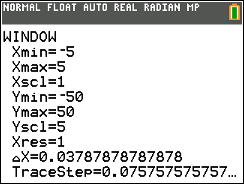
\includegraphics{hw12-2-1}

    We already know that we have a minimum at $(-2,0)$ due to the even
    multiplicity. The other extrema are found as follows:
    
    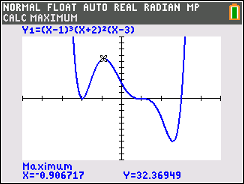
\includegraphics{hw12-2-2}

    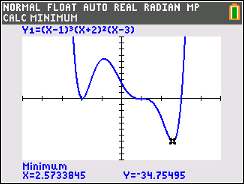
\includegraphics{hw12-2-3}
    
  \end{enumerate}
  
\end{enumerate}
\end{document}
